\documentclass{standalone}
\usepackage{tikz}
\usepackage{xcolor}
\usetikzlibrary{patterns, positioning}
\usetikzlibrary{shapes.misc}
\usepackage[outline]{contour}
\contourlength{1.5pt} 


\begin{document}
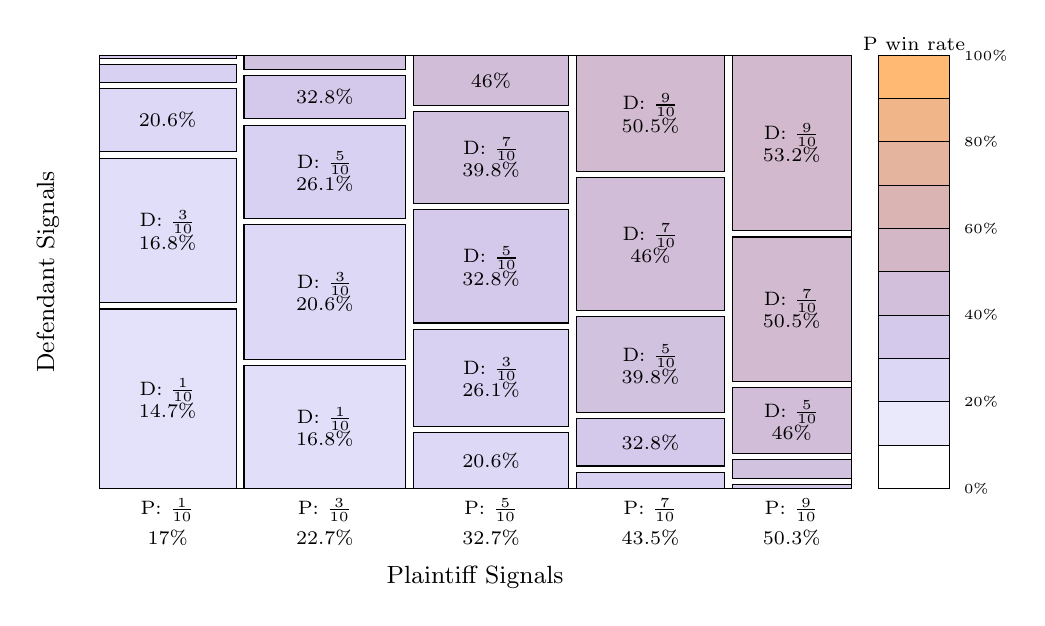
\begin{tikzpicture}
\newcommand{\DFractionOffset}{0.4}
\newcommand{\AxisLabelYAdjust}{-0.235}
\draw[draw=black] (0.6,2) rectangle (10.15,7.5);
\draw[fill=blue!85!orange!15!white!83!white, draw=black] (0.6,2) rectangle (2.3396,4.2789);
\draw (1.4698225061586938, 3.1394275505596037) node[font=\scriptsize, text=black, align=center] {D: $\frac{1}{10}$\\ 14.7\%};
\draw[fill=blue!83!orange!17!white!82!white, draw=black] (0.6,4.3589) rectangle (2.3396,6.1943);
\draw (1.4698225061586938, 5.276558168882577) node[font=\scriptsize, text=black, align=center] {D: $\frac{3}{10}$\\ 16.8\%};
\draw[fill=blue!79!orange!21!white!81!white, draw=black] (0.6,6.2743) rectangle (2.3396,7.0795);
\draw (1.4698225061586938, 6.676860120382227) node[font=\scriptsize, text=black, align=center] {20.6\%};
\draw[fill=blue!74!orange!26!white!79!white, draw=black] (0.6,7.1595) rectangle (2.3396,7.3795);
\draw[fill=blue!67!orange!33!white!77!white, draw=black] (0.6,7.4595) rectangle (2.3396,7.5);
\draw (1.4698225061586938, 1.6) node[anchor=north, font=\scriptsize, text=black] {17\%};
\draw (1.4698225061586938, {1.6 + \DFractionOffset}) node[anchor=north, font=\scriptsize, text=black] {P: $\frac{1}{10}$};
\draw[fill=blue!83!orange!17!white!82!white, draw=black] (2.4396,2) rectangle (4.4916,3.556);
\draw (3.4656370384720705, 2.7780165556482697) node[font=\scriptsize, text=black, align=center] {D: $\frac{1}{10}$\\ 16.8\%};
\draw[fill=blue!79!orange!21!white!81!white, draw=black] (2.4396,3.636) rectangle (4.4916,5.3524);
\draw (3.4656370384720705, 4.494215710530173) node[font=\scriptsize, text=black, align=center] {D: $\frac{3}{10}$\\ 20.6\%};
\draw[fill=blue!74!orange!26!white!79!white, draw=black] (2.4396,5.4324) rectangle (4.4916,6.6141);
\draw (3.4656370384720705, 6.023236573769449) node[font=\scriptsize, text=black, align=center] {D: $\frac{5}{10}$\\ 26.1\%};
\draw[fill=blue!67!orange!33!white!77!white, draw=black] (2.4396,6.6941) rectangle (4.4916,7.2438);
\draw (3.4656370384720705, 6.968961071579145) node[font=\scriptsize, text=black, align=center] {32.8\%};
\draw[fill=blue!60!orange!40!white!75!white, draw=black] (2.4396,7.3238) rectangle (4.4916,7.5);
\draw (3.4656370384720705, 1.6) node[anchor=north, font=\scriptsize, text=black] {22.7\%};
\draw (3.4656370384720705, {1.6 + \DFractionOffset}) node[anchor=north, font=\scriptsize, text=black] {P: $\frac{3}{10}$};
\draw[fill=blue!79!orange!21!white!81!white, draw=black] (4.5916,2) rectangle (6.5628,2.7106);
\draw (5.577194815687055, 2.3553183231574746) node[font=\scriptsize, text=black, align=center] {20.6\%};
\draw[fill=blue!74!orange!26!white!79!white, draw=black] (4.5916,2.7906) rectangle (6.5628,4.0208);
\draw (5.577194815687055, 3.4057101175315583) node[font=\scriptsize, text=black, align=center] {D: $\frac{3}{10}$\\ 26.1\%};
\draw[fill=blue!67!orange!33!white!77!white, draw=black] (4.5916,4.1008) rectangle (6.5628,5.5401);
\draw (5.577194815687055, 4.820465220673054) node[font=\scriptsize, text=black, align=center] {D: $\frac{5}{10}$\\ 32.8\%};
\draw[fill=blue!60!orange!40!white!75!white, draw=black] (4.5916,5.6201) rectangle (6.5628,6.7818);
\draw (5.577194815687055, 6.200976223319583) node[font=\scriptsize, text=black, align=center] {D: $\frac{7}{10}$\\ 39.8\%};
\draw[fill=blue!54!orange!46!white!73!white, draw=black] (4.5916,6.8618) rectangle (6.5628,7.5);
\draw (5.577194815687055, 7.180902797020614) node[font=\scriptsize, text=black, align=center] {46\%};
\draw (5.577194815687055, 1.6) node[anchor=north, font=\scriptsize, text=black] {32.7\%};
\draw (5.577194815687055, {1.6 + \DFractionOffset}) node[anchor=north, font=\scriptsize, text=black] {P: $\frac{5}{10}$};
\draw[fill=blue!74!orange!26!white!79!white, draw=black] (6.6628,2) rectangle (8.541,2.2038);
\draw[fill=blue!67!orange!33!white!77!white, draw=black] (6.6628,2.2838) rectangle (8.541,2.8844);
\draw (7.601884915266196, 2.584100710976728) node[font=\scriptsize, text=black, align=center] {32.8\%};
\draw[fill=blue!60!orange!40!white!75!white, draw=black] (6.6628,2.9644) rectangle (8.541,4.1835);
\draw (7.601884915266196, 3.573965970378709) node[font=\scriptsize, text=black, align=center] {D: $\frac{5}{10}$\\ 39.8\%};
\draw[fill=blue!54!orange!46!white!73!white, draw=black] (6.6628,4.2635) rectangle (8.541,5.9475);
\draw (7.601884915266196, 5.105513715646682) node[font=\scriptsize, text=black, align=center] {D: $\frac{7}{10}$\\ 46\%};
\draw[fill=blue!49!orange!51!white!71!white, draw=black] (6.6628,6.0275) rectangle (8.541,7.5);
\draw (7.601884915266196, 6.763754512113077) node[font=\scriptsize, text=black, align=center] {D: $\frac{9}{10}$\\ 50.5\%};
\draw (7.601884915266196, 1.6) node[anchor=north, font=\scriptsize, text=black] {43.5\%};
\draw (7.601884915266196, {1.6 + \DFractionOffset}) node[anchor=north, font=\scriptsize, text=black] {P: $\frac{7}{10}$};
\draw[fill=blue!67!orange!33!white!77!white, draw=black] (8.641,2) rectangle (10.15,2.0467);
\draw[fill=blue!60!orange!40!white!75!white, draw=black] (8.641,2.1267) rectangle (10.15,2.3662);
\draw[fill=blue!54!orange!46!white!73!white, draw=black] (8.641,2.4462) rectangle (10.15,3.2799);
\draw (9.395504631892518, 2.863072293342459) node[font=\scriptsize, text=black, align=center] {D: $\frac{5}{10}$\\ 46\%};
\draw[fill=blue!49!orange!51!white!71!white, draw=black] (8.641,3.3599) rectangle (10.15,5.1927);
\draw (9.395504631892518, 4.2763042536665195) node[font=\scriptsize, text=black, align=center] {D: $\frac{7}{10}$\\ 50.5\%};
\draw[fill=blue!47!orange!53!white!70!white, draw=black] (8.641,5.2727) rectangle (10.15,7.5);
\draw (9.395504631892518, 6.386356440198403) node[font=\scriptsize, text=black, align=center] {D: $\frac{9}{10}$\\ 53.2\%};
\draw (9.395504631892518, 1.6) node[anchor=north, font=\scriptsize, text=black] {50.3\%};
\draw (9.395504631892518, {1.6 + \DFractionOffset}) node[anchor=north, font=\scriptsize, text=black] {P: $\frac{9}{10}$};
\node[font=\small, text=black] at (5.375, {1.1 + \AxisLabelYAdjust}) {Plaintiff Signals};
\node[font=\small, text=black, rotate=90] at (-0.050000000000000044, 4.75) {Defendant Signals};
\draw[draw=black] (10.5,2) rectangle (11.4,7.5);
\draw (10.95, 7.65) node[font=\scriptsize, text=black] {P win rate};
\draw[fill=blue!100!orange!0!white!88!white, draw=black] (10.5,2) rectangle (11.4,2.55);
\draw[fill=blue!89!orange!11!white!84!white, draw=black] (10.5,2.55) rectangle (11.4,3.1);
\draw[fill=blue!78!orange!22!white!81!white, draw=black] (10.5,3.1) rectangle (11.4,3.65);
\draw[fill=blue!67!orange!33!white!77!white, draw=black] (10.5,3.65) rectangle (11.4,4.2);
\draw[fill=blue!56!orange!44!white!73!white, draw=black] (10.5,4.2) rectangle (11.4,4.75);
\draw[fill=blue!44!orange!56!white!70!white, draw=black] (10.5,4.75) rectangle (11.4,5.3);
\draw[fill=blue!33!orange!67!white!66!white, draw=black] (10.5,5.3) rectangle (11.4,5.85);
\draw[fill=blue!22!orange!78!white!62!white, draw=black] (10.5,5.85) rectangle (11.4,6.4);
\draw[fill=blue!11!orange!89!white!59!white, draw=black] (10.5,6.4) rectangle (11.4,6.95);
\draw[fill=blue!0!orange!100!white!55!white, draw=black] (10.5,6.95) rectangle (11.4,7.5);
\draw (11.46, 2) node[anchor=west, font=\tiny, text=black] {0\%};
\draw (11.46, 3.1) node[anchor=west, font=\tiny, text=black] {20\%};
\draw (11.46, 4.2) node[anchor=west, font=\tiny, text=black] {40\%};
\draw (11.46, 5.3) node[anchor=west, font=\tiny, text=black] {60\%};
\draw (11.46, 6.4) node[anchor=west, font=\tiny, text=black] {80\%};
\draw (11.46, 7.5) node[anchor=west, font=\tiny, text=black] {100\%};


\end{tikzpicture}
\end{document}